%****************************************************************************%
%* DIET User's Manual: DIET forwarders                                                *%
%*                                                                          *%
%*  Author(s):                                                              *%
%*    - Gaël Le Mahec                                                       *%
%*                                                                          *%
%* $LICENSE$                                                                *%
%****************************************************************************%
%* $Id$
%* $Log$
%* Revision 1.4  2010/10/26 01:45:03  bdepardo
%* Typos
%*
%* Revision 1.3  2010/10/25 08:30:05  bdepardo
%* Explanation on -C option which is mandatory to create the connection.
%*
%* Revision 1.2  2010/09/10 13:05:29  bdepardo
%* Typos
%*
%* Revision 1.1  2010/09/10 11:47:21  glemahec
%* The missing file...
%*
%****************************************************************************%
\chapter{\diet forwarders}
\label{ch:forwarders}
The \diet middleware uses CORBA as its communication layer. It is an easy
and flexible way for the different platform components to communicate.
However, deploying \diet on heterogeneous networks that are not
reachable from each other except through ssh connection is a complicated
task needing complex configuration. Moreover, to ensure that all
objects can contact each others, we need to set-up and launch ssh
tunnels between each of them, reducing significantly the \diet
scalability in that network configuration context.

The \textit{\diet forwarders} are the solution for such a situation, by
reducing the number of ssh tunnels to the minimum and making their
launch totally transparent for the final users. The \diet forwarders
configuration is very simple even for very complex network topologies.

The next section presents the global operation of \diet
forwarders. Section \ref{sec:ForwarderConfig} presents the \dietforwarder
executable, its command-line options and configuration file. Then,
section \ref{sec:ForwarderExamples} gives two examples of forwarder
configurations.

\section{Easy CORBA objects connections through ssh}
Each CORBA object in \diet is reachable through omniORB using a TCP
port and the hostname of the machine on which it is executed. By
default these parameters are fixed automatically by omniORB but it is
also possible to choose them statically using the \diet configuration
file.
When two objects are located on different networks that are reachable
only through ssh, it is easy to open an ssh tunnel to redirect the
communications between them on the good port and host. Then, correcting
the objects bindings into the omniNames servers is sufficient to ensure
the communications between the different objects. To allow two
CORBA objects to communicate through an ssh tunnel, users must:
\begin{itemize}
\item Start the process which declares the objects and register them
  into the omniNames server(s).
\item Open ssh tunnels that redirect the local objects ports to
  remote ports.
\item Modify the objects bindings in the omniNames server(s) to make
  them point to the forwarded ports.
\end{itemize}

When using few objects that do not need much interaction, these steps
can easily be done ``manually''. But \diet uses several different
objects for each element and is designed to manage thousands of nodes.
Moreover, creating an ssh tunnel between all the nodes of a Grid
cannot even be considered.

The \diet forwarders deal with this problem by creating \textit{proxy
  objects} that forward the communications to a peer forwarder through
a unique ssh tunnel. Then, only one ssh tunnel is created to connect
two different networks. This system also allows users to define complex
communications routing. Figure \ref{fig:forwarder} shows how the \diet
forwarders work to route communications through ssh tunnels. Moreover
most of the configuration of the forwarders automatically can be set
by \diet itself.

\begin{figure}[htp]
\begin{center}
  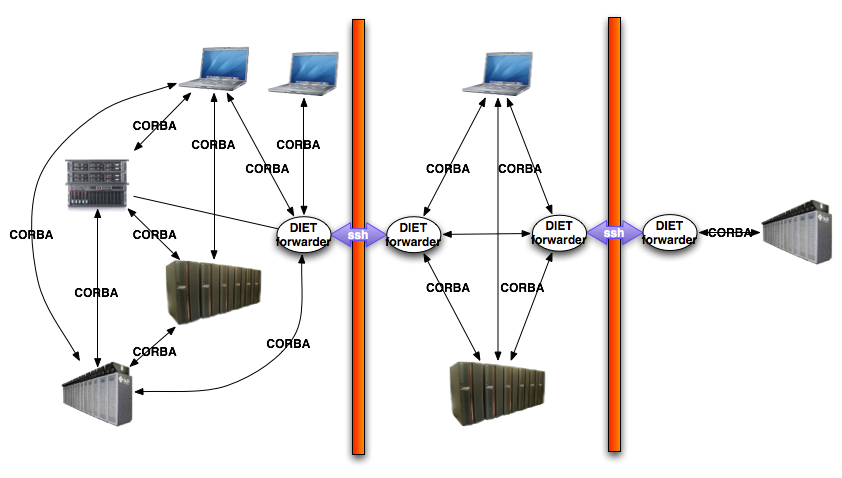
\includegraphics[width=12cm]{fig/Forwarder}
\end{center}
\caption{Forwarders routing \diet communication through ssh tunnels
  \label{fig:forwarder}}
\end{figure}

\section{The \dietforwarder executable}
\label{sec:ForwarderConfig}
Since \diet 2.5, when installing \diet, an executable called \textit{DIETForwarder}
is installed on the \textit{bin} directory. It allows to launch a
forwarder object following the configuration passed on the command
line.
\subsection{Command line options}
The \diet forwarder executable takes several options to be launched:
\begin{itemize}
\item \verb#--name#: to define the name of the forwarder.
\item \verb#--peer-name#: the name of its peer on the other network.
\item \verb#--ssh-host#: the ssh host for the tunnel creation.
\item \verb#--ssh-port#: the port to use to establish the ssh
  connection (by default: 22).
\item \verb#--ssh-login#: the login to use to establish the ssh
  connection (by default: current user login).
\item \verb#--ssh-key#: the private key to use to establish the ssh
  connection (by default: \verb#$HOME/.ssh/id_rsa#).
\item \verb#--remote-port#: the port to listen on the ssh host.
\item \verb#--net-config#: the path to the configuration file.
\item \verb#-C#: create the tunnel from this forwarder.
\end{itemize}
The remote port can be chosen randomly among the available TCP ports
on the remote host.\\

\noindent In order, to activate a \diet forwarder, users must:
\begin{itemize}
\item Launch omniNames on the remote and local hosts.
\item Launch the first peer on the remote host, only defining its name
  and its network configuration.
\item Launch the second peer, passing it it the first peer name, the
  ssh connection informations, the remote port to use and its network
  configuration, and the \verb#-C# option to force it to create the
  ssh tunnel.
\end{itemize}

\noindent\textit{Rem: The forwarders must be launched before the \diet
  hierarchy.}


\subsection{Configuration file}
To describe to which networks a forwarder gives an access to, users pass a
configuration file to the executable through the \verb#--net-config#
option. This file contains several rules describing which network is
reachable using this forwarder:
\begin{itemize}
\item The \verb#accept# rules: these rules describe which network can
  be accessed using the forwarder.
\item The \verb#reject# rules: these rules describe which network
  cannot be accessed using the forwarder.\\
\end{itemize}

A rule is a regular expression that describes a set of hostnames or IP
addresses. \textit{localhost} is a special rule that represent, the
``localhost'' string, but also the 127.0.0.1 IP address and the main
network interface IP addresses.\\

A \diet forwarder configuration file line always starts with
\textit{accept:} or \textit{reject:} immediately followed by a regular
expression.\\

The rules are evaluated starting by the \textit{accept} rules. Then
the rule \textit{accept:.*} (accept every hostname) followed by the
rule \textit{reject:localhost} means that the forwarder manage the
connections to every hosts except the local host.

Examples of configuration files are given in section
\ref{sec:ForwarderExamples}.


\section{Configuration examples}
\label{sec:ForwarderExamples}
The first example presents the configurations of \diet forwarders to
connect a \sed located on a network only reachable through ssh to a
\diet hierarchy located on another network.\\

The second example presents the configurations of \diet forwarders to
connect three networks: the first one can only reach the second one
through ssh and the third one can also only reach the second one
through ssh. We want to connect \diet elements distributed over the
three networks.
\subsection{Simple configuration}
\begin{itemize}
\item The two different domains are \textit{net1} and \textit{net2}. The forwarders will
  be launched on the hosts \textit{fwd.net1} and \textit{fwd.net2}.
\item There is no possibility to access \textit{fwd.net1} from
  \textit{fwd.net2} but users can access \textit{fwd.net2} from
  \textit{fwd.net1} using an ssh connection.
\item The forwarder on \textit{fwd.net1} is named \textit{Fwd1}, the
  forwarder on \textit{fwd.net2} is named \textit{Fwd2}.
\item One \sed is launched on \textit{fwd.net2}, the rest of the \diet
  hierarchy is launched on the \textit{net1} domain.\\
\end{itemize}

\noindent\textbf{Command line to launch \textit{Fwd1}: }\\
{\small \it fwd.net1\$ dietForwarder {\tiny$--$}name Fwd1
  {\tiny$--$}peer-name Fwd2 $\backslash$\\
  \hspace*{4.2cm}{\tiny$--$}ssh-host fwd.net2 {\tiny$--$}ssh-login
  dietUser $\backslash$\\
  \hspace*{4.2cm}{\tiny$--$}ssh-key id\_rsa\_net2
  {\tiny$--$}remote-port 50000 $\backslash$\\
  \hspace*{4.2cm}{\tiny$--$}net-config net1.cfg {\tiny$-$}C}\\[2mm]
\noindent\textbf{Command line to launch \textit{Fwd2}: }\\
{\small \it fwd.net2\$ dietForwarder {\tiny$--$}name Fwd2
  {\tiny$--$}net-config net2.cfg}\\[3mm]
\noindent\textbf{Configuration file for \textit{Fwd1}:}\\
In this example, the forwarders \textit{Fwd1} accepts only the
connections to \textit{fwd.net2}.
\begin{verbatim}
accept:fwd.net2
\end{verbatim}

\noindent\textbf{Configuration file for \textit{Fwd2}:}\\
In this example, the forwarders \textit{Fwd2} accepts all the
connections except those which are for the localhost.
\begin{verbatim}
accept:.*
reject:localhost
\end{verbatim}

Note that \textit{Fwd2} has to be launched before \textit{Fwd1}.
When the two forwarders are launched, the user can deploy his \diet
hierarchy. All the communications through  \diet forwarders are
transparent.

\subsection{Complex network topology}
To connect the three domains, we need 4 forwarders (2 pairs): one on
\textit{net1}, two on \textit{net2} and one on \textit{net3}.
\begin{itemize}
\item The three domains are: \textit{net1}, \textit{net2} and
  \textit{net3}.
\item The machines located on \textit{net1} and \textit{net3} are only
  reachable from \textit{fwd.net2} through ssh.
\item The four forwarders are named \textit{Fwd1}, \textit{Fwd2-1},
  \textit{Fwd2-3} and \textit{Fwd3}.
\item The \diet hierarchy is distributed on the three networks.\\
\end{itemize}

\noindent\textbf{Command line to launch \textit{Fwd1}: }\\
{\small \it fwd.net1\$ dietForwarder {\tiny$--$}name Fwd1
  {\tiny$--$}net-config net1.cfg}\\[2mm]

\noindent\textbf{Command line to launch \textit{Fwd2-1}: }\\
{\small \it fwd.net2\$ dietForwarder {\tiny$--$}name Fwd2-1
  {\tiny$--$}peer-name Fwd1 $\backslash$\\
  \hspace*{4.2cm}{\tiny$--$}ssh-host fwd.net1 {\tiny$--$}ssh-login
  dietUser $\backslash$\\
  \hspace*{4.2cm}{\tiny$--$}ssh-key id\_rsa\_net1
  {\tiny$--$}remote-port 50000 $\backslash$\\
  \hspace*{4.2cm}{\tiny$--$}net-config net2-1.cfg {\tiny$-$}C}\\[2mm]

\noindent\textbf{Command line to launch \textit{Fwd2-3}: }\\
{\small \it fwd.net2\$ dietForwarder {\tiny$--$}name Fwd2-3
  {\tiny$--$}peer-name Fwd3 $\backslash$\\
  \hspace*{4.2cm}{\tiny$--$}ssh-host fwd.net3 {\tiny$--$}ssh-login
  dietUser $\backslash$\\
  \hspace*{4.2cm}{\tiny$--$}ssh-key id\_rsa\_net3
  {\tiny$--$}remote-port 50000 $\backslash$\\
  \hspace*{4.2cm}{\tiny$--$}net-config net2-3.cfg {\tiny$-$}C}\\[2mm]

\noindent\textbf{Command line to launch \textit{Fwd3}: }\\
{\small \it fwd.net3\$ dietForwarder {\tiny$--$}name Fwd3
  {\tiny$--$}net-config net3.cfg}\\[3mm]

\noindent\textbf{Configuration file for \textit{Fwd1}:}\\
\textit{Fwd1} manages the communications for all the host outside
\textit{net1}.
\begin{verbatim}
accept:.*
reject:.*\.net1
\end{verbatim}

\noindent\textbf{Configuration file for \textit{Fwd2-1}:}\\
\textit{Fwd2-1} manages the communication for all the hosts located on
\textit{net1}.
\begin{verbatim}
accept:.*\.net1
\end{verbatim}

\noindent\textbf{Configuration file for \textit{Fwd2-3}:}\\
\textit{Fwd2-3} manages the communication for all the hosts located on
\textit{net3}.
\begin{verbatim}
accept:.*\.net3
\end{verbatim}

\noindent\textbf{Configuration file for \textit{Fwd3}:}\\
\textit{Fwd1} manages the communications for all the host outside
\textit{net3}.
\begin{verbatim}
accept:.*
reject:.*\.net3
\end{verbatim}

Using this configuration, a communication from a host on \textit{net1}
to a host on \textit{net3} is first routed from \textit{Fwd1} to
\textit{Fwd2-1} and then from \textit{Fwd2-3} to \textit{Fwd3}.
Note that \textit{Fwd1} has to be launched before \textit{Fwd2-1}, and
\textit{Fwd3} has to be launched before \textit{Fwd2-3}.